
在前面的章节中，我们讨论了配分函数如何描述系统的热力学性质，以及 AdS/CFT 对偶如何将引力理论与量子场论联系起来。现在我们转向一个在现代物理学中越来越重要的概念：纠缠熵。纠缠熵度量量子系统中子系统之间的纠缠程度，它在量子信息理论、凝聚态物理和高能物理中都有重要应用。在 AdS/CFT 对偶中，纠缠熵有一个几何解释：它可以通过计算体空间中极小曲面的面积来得到，这就是著名的 Ryu-Takayanagi 公式~\cite{Ryu2006}。

%=============================================================================
\section{量子纠缠的基本概念}
%=============================================================================

要理解纠缠熵，我们首先需要理解量子纠缠。量子纠缠是量子力学中最反直觉的现象之一：两个粒子可以处于一种"纠缠"状态，即使它们相距很远，对其中一个粒子的测量会瞬间影响另一个粒子的状态。下面我们从复合系统的数学结构出发，给出量子纠缠的严格定义。

\begin{definition}[复合系统与张量积]
考虑一个由两个子系统 $A$ 和 $B$ 组成的量子系统。系统的总希尔伯特空间可以分解为
\begin{equation}
    \mathcal{H}_{\rm tot} = \mathcal{H}_A \otimes \mathcal{H}_B.
\end{equation}
如果系统的状态 $|\Psi\rangle$ 可以写成两个子系统状态的张量积
\begin{equation}
    |\Psi\rangle = |\psi_A\rangle \otimes |\psi_B\rangle,
\end{equation}
那么这个状态是\textbf{可分的}（separable），不存在纠缠。
\end{definition}

图~\ref{fig:entangled_system} 展示了纠缠系统中两个子区域 $A$ 和 $B$ 的示意图。

\begin{figure}[htbp]
\centering
\begin{tikzpicture}[scale=1.2]
    % 画区域A
    \draw[thick, blue, fill=blue!8] (-2.5,-1.5) rectangle (-0.2,1.5);
    \node[blue, font=\large] at (-1.35, 1.8) {$A$};
    % 画区域B
    \draw[thick, red, fill=red!8] (0.2,-1.5) rectangle (2.5,1.5);
    \node[red, font=\large] at (1.35, 1.8) {$B$};
    % 纠缠连线
    \foreach \y in {-1.0,-0.5,0.0,0.5,1.0} {
        \draw[thick, purple, <->, >=stealth] (-0.2,\y) -- (0.2,\y);
    }
    \node[purple, font=\footnotesize] at (0, -1.8) {纠缠关联};
    % 标注Hilbert空间
    \node[font=\small] at (-1.35, -0.8) {$\mathcal{H}_A$};
    \node[font=\small] at (1.35, -0.8) {$\mathcal{H}_B$};
\end{tikzpicture}
\caption{纠缠系统示意图：子区域 $A$ 和 $B$ 构成总系统，它们通过量子纠缠（紫色连线）相关联。即使 $A$ 和 $B$ 空间分离，纠缠仍然存在。}
\label{fig:entangled_system}
\end{figure}

然而，大多数量子态不能写成这种可分形式。例如，考虑以下双量子比特态。

\begin{example}[贝尔态的纠缠]\label{ex:bell}
考虑贝尔态（Bell state）：
\begin{equation}\label{eq:bell_state}
    |\Psi^-\rangle = \frac{1}{\sqrt{2}}(|\uparrow\downarrow\rangle - |\downarrow\uparrow\rangle).
\end{equation}
我们证明这个状态不可分。假设存在 $|\psi_A\rangle = \alpha|\uparrow\rangle + \beta|\downarrow\rangle$ 和 $|\phi_B\rangle = \gamma|\uparrow\rangle + \delta|\downarrow\rangle$ 使得 $|\Psi^-\rangle = |\psi_A\rangle \otimes |\phi_B\rangle$，则
\begin{equation}
    |\psi_A\rangle \otimes |\phi_B\rangle = \alpha\gamma|\uparrow\uparrow\rangle + \alpha\delta|\uparrow\downarrow\rangle + \beta\gamma|\downarrow\uparrow\rangle + \beta\delta|\downarrow\downarrow\rangle.
\end{equation}
与~\eqref{eq:bell_state} 比较系数，必须满足 $\alpha\gamma = 0$、$\beta\delta = 0$、$\alpha\delta = 1/\sqrt{2}$、$\beta\gamma = -1/\sqrt{2}$。由 $\alpha\delta \neq 0$ 知 $\alpha \neq 0$ 且 $\delta \neq 0$，但由 $\alpha\gamma = 0$ 知 $\gamma = 0$，这与 $\beta\gamma = -1/\sqrt{2} \neq 0$ 矛盾。因此 $|\Psi^-\rangle$ 不可分，即为纠缠态。$\square$
\end{example}

四个贝尔态构成了双量子比特空间的一组正交归一基：
\begin{equation}
    |\Psi^\pm\rangle = \frac{1}{\sqrt{2}}(|\uparrow\downarrow\rangle \pm |\downarrow\uparrow\rangle), \quad
    |\Phi^\pm\rangle = \frac{1}{\sqrt{2}}(|\uparrow\uparrow\rangle \pm |\downarrow\downarrow\rangle).
\end{equation}

\begin{figure}[htbp]
\centering
\begin{tikzpicture}[scale=1.0, >=stealth]
    % 输入态
    \node at (-1, 2) {$|\uparrow\rangle$};
    \node at (-1, 0) {$|\downarrow\rangle$};
    % 线
    \draw[thick] (-0.5, 2) -- (1.5, 2);
    \draw[thick] (-0.5, 0) -- (1.5, 0);
    % H gate
    \draw[thick, fill=yellow!30] (0, 1.7) rectangle (0.6, 2.3);
    \node at (0.3, 2) {$H$};
    % CNOT
    \draw[thick, fill=green!20] (1.5, 1.7) -- (2.1, 2) -- (1.5, 2.3) -- cycle;
    \filldraw (1.8, 2) circle (2pt);
    \draw[thick] (1.8, 0) -- (1.8, 1.7);
    \draw[thick] (1.8, 0) circle (4pt);
    % 输出
    \draw[thick] (2.1, 2) -- (3.5, 2);
    \draw[thick] (1.8, 0) -- (3.5, 0);
    \node at (4.2, 2) {$\frac{1}{\sqrt{2}}(|\uparrow\rangle + |\downarrow\rangle)$};
    \node at (4.2, 0) {条件翻转};
    % 结果
    \node[font=\small] at (3.5, -1) {$\to |\Phi^+\rangle = \frac{1}{\sqrt{2}}(|\uparrow\uparrow\rangle + |\downarrow\downarrow\rangle)$};
    % 标注
    \node[font=\footnotesize] at (0.3, 2.7) {Hadamard};
    \node[font=\footnotesize] at (1.8, 2.7) {CNOT};
\end{tikzpicture}
\caption{制备贝尔态 $|\Phi^+\rangle$ 的量子线路：先对第一个量子比特施加 Hadamard 门，再以第一个比特为控制比特施加 CNOT 门。}
\label{fig:bell_circuit}
\end{figure}

\begin{remark}
量子纠缠与经典关联有本质区别。经典关联（如将一副手套分寄两地）可以通过隐变量解释，而贝尔不等式的违反表明量子纠缠无法用任何局域隐变量理论描述。
\end{remark}

%=============================================================================
\section{约化密度矩阵与纠缠熵}
%=============================================================================

在量子力学中，当我们只关注复合系统的某个子系统时，描述该子系统状态的数学工具是约化密度矩阵。为了量化纠缠程度，我们需要引入这一概念并定义纠缠熵。

\begin{definition}[密度矩阵与约化密度矩阵]
对于一个纯态 $|\Psi\rangle$，总密度矩阵为 $\rho_{\rm tot} = |\Psi\rangle\langle\Psi|$。当我们只关注子系统 $A$ 时，需要对子系统 $B$ 求偏迹（partial trace），得到约化密度矩阵：
\begin{equation}\label{eq:reduced_dm}
    \rho_A = \Tr_B(\rho_{\rm tot}) = \sum_{i} {}_B\langle i | \rho_{\rm tot} | i\rangle_B,
\end{equation}
其中 $\{|i\rangle_B\}$ 是子系统 $B$ 的一组正交归一基。
\end{definition}

下面我们对贝尔态显式计算约化密度矩阵。

\begin{example}[贝尔态的约化密度矩阵]
对于贝尔态 $|\Psi^-\rangle = \frac{1}{\sqrt{2}}(|\uparrow\downarrow\rangle - |\downarrow\uparrow\rangle)$，总密度矩阵为
\begin{equation}
    \rho_{\rm tot} = \frac{1}{2}\big(|\uparrow\downarrow\rangle - |\downarrow\uparrow\rangle\big)\big(\langle\uparrow\downarrow| - \langle\downarrow\uparrow|\big).
\end{equation}
展开得到
\begin{equation}
    \rho_{\rm tot} = \frac{1}{2}\big(|\uparrow\downarrow\rangle\langle\uparrow\downarrow| - |\uparrow\downarrow\rangle\langle\downarrow\uparrow| - |\downarrow\uparrow\rangle\langle\uparrow\downarrow| + |\downarrow\uparrow\rangle\langle\downarrow\uparrow|\big).
\end{equation}
对 $B$ 求偏迹，取 $B$ 的基为 $\{|\uparrow\rangle_B, |\downarrow\rangle_B\}$：
\begin{align}
    \rho_A &= {}_B\langle\uparrow|\rho_{\rm tot}|\uparrow\rangle_B + {}_B\langle\downarrow|\rho_{\rm tot}|\downarrow\rangle_B \nonumber\\
    &= \frac{1}{2}|\downarrow\rangle\langle\downarrow| \cdot 1 + \frac{1}{2}|\uparrow\rangle\langle\uparrow| \cdot 1 \nonumber\\
    &= \frac{1}{2}\big(|\uparrow\rangle\langle\uparrow| + |\downarrow\rangle\langle\downarrow|\big) = \frac{1}{2}\mathbb{I}_A.
\end{align}
约化密度矩阵为最大混合态 $\frac{1}{2}\mathbb{I}_A$，这表明我们对子系统 $A$ 的状态完全"无知"——它处于最大纠缠状态。
\end{example}

约化密度矩阵 $\rho_A$ 的本征值分布反映了纠缠程度。如果系统是可分的，$\rho_A$ 是纯态，只有一个本征值为 1，其余为 0；如果系统是纠缠的，$\rho_A$ 是混合态，本征值分布更加均匀。

\begin{definition}[纠缠熵]\label{def:ee}
纠缠熵定义为约化密度矩阵的 von Neumann 熵：
\begin{equation}\label{eq:ee}
    S_A = -\Tr_A(\rho_A \ln \rho_A) = -\sum_i p_i \ln p_i,
\end{equation}
其中 $p_i$ 是 $\rho_A$ 的本征值。纠缠熵度量了子系统 $A$ 与子系统 $B$ 之间的纠缠程度。
\end{definition}

\begin{proof}
公式~\eqref{eq:ee} 的推导如下。设 $\rho_A$ 的谱分解为 $\rho_A = \sum_i p_i |e_i\rangle\langle e_i|$，则
\begin{equation}
    \ln \rho_A = \sum_i (\ln p_i) |e_i\rangle\langle e_i|,
\end{equation}
从而
\begin{equation}
    \rho_A \ln \rho_A = \sum_i p_i (\ln p_i) |e_i\rangle\langle e_i|,
\end{equation}
取迹得到
\begin{equation}
    \Tr_A(\rho_A \ln \rho_A) = \sum_i p_i \ln p_i.
\end{equation}
因此 $S_A = -\sum_i p_i \ln p_i$。这里使用自然对数 $\ln$，约定 $0 \ln 0 = 0$。
\end{proof}

\begin{note}[纠缠熵的物理意义]
纠缠熵可以被理解为"我们对子系统 $A$ 的无知程度"：
\begin{itemize}
    \item 如果系统是可分的，$\rho_A$ 为纯态，$S_A = 0$。
    \item 如果系统是纠缠的，$\rho_A$ 为混合态，$S_A > 0$。
    \item 纠缠熵越大，子系统之间的纠缠越强。
    \item 对于 $d$ 维希尔伯特空间中的最大混合态 $\rho_A = \frac{1}{d}\mathbb{I}$，纠缠熵取最大值 $S_{\max} = \ln d$。
\end{itemize}
\end{note}

\begin{example}[贝尔态的纠缠熵]
对于贝尔态，$\rho_A = \frac{1}{2}\mathbb{I}_A$，本征值为 $p_1 = p_2 = \frac{1}{2}$，因此
\begin{equation}
    S_A = -\frac{1}{2}\ln\frac{1}{2} - \frac{1}{2}\ln\frac{1}{2} = \ln 2.
\end{equation}
这正好是最大值 $S_{\max} = \ln 2$（对于二维希尔伯特空间），确认了贝尔态是最大纠缠态。
\end{example}

%=============================================================================
\section{纠缠熵的基本性质}
%=============================================================================

纠缠熵具有几个重要的数学性质。这些性质的证明依赖于密度矩阵的半正定性以及 von Neumann 熵的凹性等基本工具。

\begin{property}[基本性质]\label{prop:basic}
纠缠熵满足以下基本性质：
\begin{enumerate}
    \item \textbf{非负性}：$S_A \geq 0$，等号成立当且仅当 $\rho_A$ 为纯态。
    \item \textbf{对称性}：对于纯态 $|\Psi\rangle_{AB}$，$S_A = S_B$。
    \item \textbf{上界}：$S_A \leq \ln \dim\mathcal{H}_A$。
\end{enumerate}
\end{property}

\begin{proof}[对称性的证明]
对于纯态 $|\Psi\rangle_{AB}$，总密度矩阵满足 $\rho_{\rm tot}^2 = \rho_{\rm tot}$。设 $\rho_A$ 的谱分解为 $\rho_A = \sum_i p_i |a_i\rangle\langle a_i|$。将 $|\Psi\rangle$ 按 Schmidt 分解展开：
\begin{equation}
    |\Psi\rangle = \sum_i \sqrt{p_i}\, |a_i\rangle_A \otimes |b_i\rangle_B,
\end{equation}
其中 $\{|b_i\rangle_B\}$ 是 $B$ 的一组正交归一基。类似地计算 $\rho_B = \Tr_A(\rho_{\rm tot})$：
\begin{equation}
    \rho_B = \sum_i p_i |b_i\rangle\langle b_i|.
\end{equation}
$\rho_B$ 的本征值集合与 $\rho_A$ 相同，因此 $S_B = -\sum_i p_i \ln p_i = S_A$。
\end{proof}

下面讨论纠缠熵最重要的不等式——次可加性。

\begin{theorem}[次可加性]\label{thm:subadditivity}
对于复合系统 $ABC$ 的纯态，约化密度矩阵的 von Neumann 熵满足：
\begin{equation}\label{eq:subadditivity}
    S_{AB} \leq S_A + S_B,
\end{equation}
等号成立当且仅当 $A$ 和 $B$ 不纠缠（即 $\rho_{AB} = \rho_A \otimes \rho_B$）。
\end{theorem}

\begin{proof}
定义量子互信息（mutual information）$I(A:B) = S_A + S_B - S_{AB}$。我们证明 $I(A:B) \geq 0$。

考虑复合系统 $AB$，有
\begin{equation}
    I(A:B) = S_A + S_B - S_{AB} = \Tr(\rho_A \ln \rho_A) + \Tr(\rho_B \ln \rho_B) - \Tr(\rho_{AB} \ln \rho_{AB}).
\end{equation}
利用相对熵（Kullback-Leibler divergence）$D(\rho\|\sigma) = \Tr(\rho \ln \rho - \rho \ln \sigma) \geq 0$，取 $\sigma = \rho_A \otimes \rho_B$：
\begin{align}
    D(\rho_{AB} \| \rho_A \otimes \rho_B) &= \Tr(\rho_{AB} \ln \rho_{AB}) - \Tr(\rho_{AB} \ln(\rho_A \otimes \rho_B)) \nonumber\\
    &= -S_{AB} - \Tr(\rho_{AB}(\ln \rho_A \otimes \mathbb{I}_B + \mathbb{I}_A \otimes \ln \rho_B)) \nonumber\\
    &= -S_{AB} - \Tr(\rho_A \ln \rho_A) - \Tr(\rho_B \ln \rho_B) \nonumber\\
    &= -S_{AB} - S_A - S_B = -I(A:B) \geq 0,
\end{align}
这里我们使用了 Klein 不等式（相对熵的非负性）。因此 $I(A:B) \geq 0$，即 $S_{AB} \leq S_A + S_B$。

当 $I(A:B) = 0$ 时，$D(\rho_{AB}\|\rho_A \otimes \rho_B) = 0$，由相对熵的性质知 $\rho_{AB} = \rho_A \otimes \rho_B$，即 $A$ 与 $B$ 不纠缠。
\end{proof}

\begin{theorem}[强次可加性]\label{thm:strong_subadd}
对于复合系统 $ABCD$，von Neumann 熵满足强次可加性：
\begin{equation}
    S_{ABC} + S_B \leq S_{AB} + S_{BC}.
\end{equation}
等价地，对于三个子系统 $A$、$B$、$C$：
\begin{equation}\label{eq:strong_subadd}
    S_{A \cup C} + S_{B} \leq S_{A \cup B} + S_{B \cup C}.
\end{equation}
\end{theorem}

\begin{note}[强次可加性的物理意义]
强次可加性是纠缠熵最重要的不等式之一，它反映了量子纠缠的"单调性"：纠缠不会因为局部操作而增加。这个性质在量子信息理论中被称为"纠缠单调性"，是量子纠缠理论的基础。在 AdS/CFT 中，强次可加性与体空间的量子极端面的性质密切相关，是证明量子极端面公式~\cite{Engelhardt2015} 的关键工具。
\end{note}

%=============================================================================
\section{面积律与量子场论}
%=============================================================================

在量子场论中，纠缠熵的一个核心性质是面积律：纠缠熵正比于子区域边界的面积，而非子区域的体积。这一性质深刻地联系了量子信息与引力物理~\cite{Casini2017}。

\begin{theorem}[面积律]\label{thm:area_law}
在 $d$ 维时空的量子场论中，对于一个空间区域 $A$，纠缠熵满足面积律：
\begin{equation}\label{eq:area_law}
    S_A = c_1 \frac{\operatorname{Area}(\partial A)}{\epsilon^{d-2}} + c_2 \frac{\operatorname{Area}(\partial A)}{\epsilon^{d-4}} + \cdots + c_{d-2}\operatorname{Area}(\partial A) \ln\frac{1}{\epsilon} + O(\epsilon^0),
\end{equation}
其中 $\epsilon$ 是紫外截断（UV cutoff），$c_i$ 是与理论细节有关的常数，$\partial A$ 是区域 $A$ 的边界。
\end{theorem}

\begin{figure}[htbp]
\centering
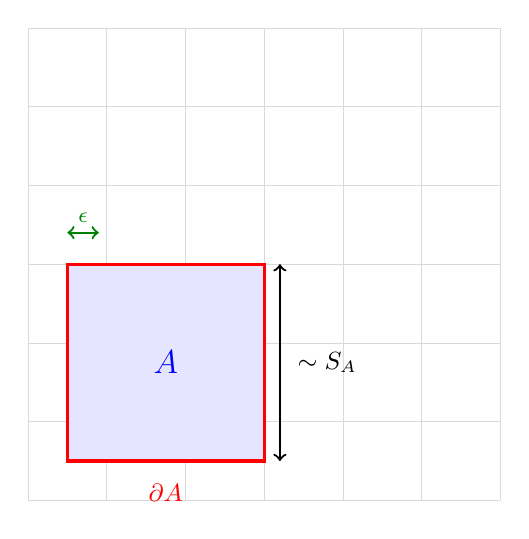
\begin{tikzpicture}[scale=1.0]
    % 网格（体区域）
    \draw[gray!30, very thin] (-3,-3) grid (3,3);
    % 区域A
    \draw[thick, blue, fill=blue!10] (-2.5,-2.5) rectangle (0,0);
    \node[blue, font=\large] at (-1.25, -1.25) {$A$};
    % 边界 partial A（加粗高亮）
    \draw[very thick, red] (-2.5, -2.5) -- (0, -2.5) -- (0, 0) -- (-2.5, 0) -- cycle;
    \node[red, font=\small] at (-1.25, -2.9) {$\partial A$};
    % 标注面积律
    \draw[<->, thick] (0.2, -2.5) -- (0.2, 0);
    \node[right, font=\small] at (0.3, -1.25) {$\sim S_A$};
    % 紫外截断
    \draw[thick, green!50!black, <->] (-2.5, 0.4) -- (-2.1, 0.4);
    \node[above, font=\footnotesize, green!50!black] at (-2.3, 0.4) {$\epsilon$};
\end{tikzpicture}
\caption{面积律示意图：纠缠熵 $S_A$ 正比于区域 $A$ 的边界 $\partial A$ 的面积（红色粗线），而非区域 $A$ 的体积。$\epsilon$ 为晶格间距或紫外截断。}
\label{fig:area_law}
\end{figure}

下面我们以自由标量场论为例，给出面积律的一个具体证明思路~\cite{Casini2017}。

\begin{proof}[自由标量场论中面积律的证明（概要）]
考虑 $d$ 维时空中自由实标量场 $\phi(x)$，空间为 $\mathbb{R}^{d-1}$，将空间分为区域 $A$ 和其补集 $\bar{A}$。

\textbf{第一步：等时关联函数。}自由场的等时关联函数为
\begin{equation}
    \langle\phi(\mathbf{x})\phi(\mathbf{y})\rangle = C(\mathbf{x}-\mathbf{y}) = \int \frac{d^{d-2}k}{(2\pi)^{d-2}} \frac{1}{2|\mathbf{k}|} e^{i\mathbf{k}\cdot(\mathbf{x}-\mathbf{y})},
\end{equation}
其中 $|\mathbf{k}| = \sqrt{k_1^2 + \cdots + k_{d-2}^2 + m^2}$。

\textbf{第二步：关联矩阵。}定义关联矩阵 $C_{AB}$，其元素为 $C_{ij} = C(\mathbf{x}_i - \mathbf{y}_j)$，其中 $\mathbf{x}_i \in A$，$\mathbf{y}_j \in A$。纠缠熵可以通过关联矩阵的本征值 $\lambda_i$ 来表达。

\textbf{第三步：纠缠熵公式。}对于高斯态，纠缠熵为
\begin{equation}
    S_A = \sum_i \left[\left(\lambda_i + \frac{1}{2}\right)\ln\left(\lambda_i + \frac{1}{2}\right) - \left(\lambda_i - \frac{1}{2}\right)\ln\left(\lambda_i - \frac{1}{2}\right)\right].
\end{equation}

\textbf{第四步：面积律的出现。}关联函数 $C(\mathbf{x}-\mathbf{y})$ 在 $\mathbf{x} \to \mathbf{y}$ 时有短距离发散 $\sim |\mathbf{x}-\mathbf{y}|^{-(d-2)}$。这一发散仅在边界 $\partial A$ 附近的点对 $(\mathbf{x}_i, \mathbf{y}_j)$ 产生主要贡献（当 $\mathbf{x}_i$ 和 $\mathbf{y}_j$ 分别位于 $A$ 和 $\bar{A}$ 时）。因此，求和的主要贡献来自边界附近的模式，给出
\begin{equation}
    S_A \sim \frac{\operatorname{Area}(\partial A)}{\epsilon^{d-2}}.
\end{equation}
这完成了面积律的证明概要。
\end{proof}

\begin{remark}
面积律的物理直观是：纠缠主要由边界附近的短程关联贡献。远离边界的内部模式对 $A$ 和 $\bar{A}$ 的关联没有净贡献，因为它们在两边对称地衰减。这一图像与凝聚态物理中一维系统的面积律（对数修正）~\cite{Calabrese2004} 一致。
\end{remark}

%=============================================================================
\section{Rényi 熵与纠缠熵的计算}
%=============================================================================

在实际计算中，直接计算 von Neumann 熵通常比较困难。一个更方便的工具是 Rényi 熵，它通过 replica trick 将熵的计算转化为配分函数的计算。

\begin{definition}[Rényi 熵]\label{def:renyi}
Rényi 熵定义为：
\begin{equation}\label{eq:renyi}
    S_n = \frac{1}{1-n} \ln \Tr_A(\rho_A^n),
\end{equation}
其中 $n$ 是正整数。
\end{definition}

\begin{proof}[Rényi 熵与 von Neumann 熵的关系]
当 $n \to 1$ 时，Rényi 熵趋于 von Neumann 熵。设 $\rho_A$ 的本征值为 $\{p_i\}$，则
\begin{equation}
    \Tr_A(\rho_A^n) = \sum_i p_i^n.
\end{equation}
当 $n \to 1$ 时，令 $n = 1 + \delta$，$\delta \to 0$：
\begin{align}
    \Tr_A(\rho_A^{1+\delta}) &= \sum_i p_i^{1+\delta} = \sum_i p_i \cdot p_i^\delta = \sum_i p_i \cdot e^{\delta \ln p_i} \nonumber\\
    &= \sum_i p_i(1 + \delta \ln p_i + O(\delta^2)) = 1 + \delta \sum_i p_i \ln p_i + O(\delta^2).
\end{align}
因此
\begin{equation}
    S_n = \frac{1}{1-n}\ln\Tr_A(\rho_A^n) = \frac{1}{-\delta}\ln\left(1 + \delta\sum_i p_i \ln p_i + O(\delta^2)\right) \to -\sum_i p_i \ln p_i = S.
\end{equation}
\end{proof}

Rényi 熵的一个重要性质是关于 $n$ 的单调性。

\begin{property}[Rényi 熵的单调性]
对于 $m > n \geq 1$，有 $S_m \leq S_n$。特别地，$S_1 = S \leq S_n$ 对所有 $n > 1$ 成立。
\end{property}

\begin{proof}
这是 Hölder 不等式的一个直接推论。定义 $f(n) = \frac{1}{1-n}\ln\Tr(\rho^n)$，可以证明 $\frac{df}{dn} \leq 0$。
\end{proof}

%=============================================================================
\section{纠缠熵与配分函数的联系}
%=============================================================================

纠缠熵可以通过配分函数来表达，这一联系在 AdS/CFT 对偶中至关重要，它将 von Neumann 熵的计算转化为复流形上路径积分的计算。

\begin{definition}[$n$ 叶黎曼面]
$n$ 叶黎曼面 $\Sigma_n$ 是一个由 $n$ 份时空副本沿着子区域 $A$ 的世界片（worldsheet）粘合而成的复流形。在 $A$ 的边界 $\partial A$ 处，副本按循环方式连接：第 $k$ 叶的 $A$ 区域与第 $k+1$ 叶的 $A$ 区域相连（$k = 1, \ldots, n$，模 $n$）。
\end{definition}

\begin{theorem}[纠缠熵与配分函数的联系]\label{thm:partition_function}
考虑 $n$ 叶黎曼面 $\Sigma_n$ 上的配分函数 $Z_n$。Rényi 熵可以写为：
\begin{equation}\label{eq:renyi_partition}
    S_n = \frac{1}{1-n} \ln \frac{Z_n}{Z_1^n},
\end{equation}
其中 $Z_1$ 是通常的配分函数。
\end{theorem}

\begin{proof}
$\Tr_A(\rho_A^n)$ 可以理解为在 $n$ 个副本之间"循环"地传播场构型。在路径积分语言中，这对应于在 $n$ 叶黎曼面上计算配分函数。具体地：
\begin{equation}
    \Tr_A(\rho_A^n) = \frac{Z_n}{Z_1^n},
\end{equation}
其中分母 $Z_1^n$ 是归一化因子，确保 $\Tr(\rho_A) = 1$。代入 Rényi 熵的定义~\eqref{eq:renyi}，得到~\eqref{eq:renyi_partition}。
\end{proof}

\begin{note}[物理意义]
这个联系的物理意义是：纠缠熵可以通过计算复几何上的配分函数来得到。在 AdS/CFT 对偶中，$n$ 叶黎曼面 $\Sigma_n$ 作为边界条件，对应于体空间中的某种复几何。通过 saddle point 近似，$Z_n$ 由体空间中的经典解主导，这为全息纠缠熵的计算提供了基础。
\end{note}

取 $n \to 1$ 极限，von Neumann 熵为
\begin{equation}
    S = -\left.\frac{\partial}{\partial n}\right|_{n=1} \ln \frac{Z_n}{Z_1^n} = -\left.\frac{\partial}{\partial n}\right|_{n=1} \ln Z_n + \ln Z_1.
\end{equation}

%=============================================================================
\section{全息纠缠熵}
%=============================================================================

AdS/CFT 对偶中，纠缠熵有一个深刻的几何解释。Ryu 和 Takayanagi 在 2006 年提出了一个著名的公式~\cite{Ryu2006}，将边界场论的纠缠熵与体空间中的极小曲面面积联系起来。

\begin{theorem}[Ryu-Takayanagi 公式]\label{thm:RT}
设 $A$ 是共形场论边界上的一个空间区域，$\gamma_A$ 是体空间中以 $\partial A$ 为边界的极小曲面（即面积泛函的临界点）。则区域 $A$ 的纠缠熵为：
\begin{equation}\label{eq:RT}
    S_A = \frac{\operatorname{Area}(\gamma_A)}{4G_N},
\end{equation}
其中 $G_N$ 是体空间中的牛顿引力常数。
\end{theorem}

\begin{remark}
Ryu-Takayanagi 公式~\eqref{eq:RT} 与黑洞熵的 Bekenstein-Hawking 公式 $S = A/(4G_N)$ 在形式上完全一致。这暗示纠缠熵与引力之间存在深刻的联系。
\end{remark}

RT 公式的证明需要利用~\eqref{eq:renyi_partition} 以及 AdS/CFT 中配分函数的引力对偶。当 $n \to 1$ 时，$n$ 叶黎曼面的引力配分函数由一个以 $\gamma_A$ 为固定边界的极值面主导，其作用量正比于 $\operatorname{Area}(\gamma_A)/(4G_N)$。

\begin{definition}[纠缠楔]
设 $\gamma_A$ 是体空间中的极小曲面，$\gamma_A$ 与边界区域 $A$ 共同围成的体空间区域 $\mathcal{W}_A$ 称为区域 $A$ 的\textbf{纠缠楔}（entanglement wedge）。
\end{definition}

\begin{figure}[htbp]
\centering
\begin{tikzpicture}[scale=1.2]
    % AdS边界
    \draw[very thick] (-3,0) arc (180:0:3);
    \node[above] at (0,3.1) {CFT 边界};
    % 区域A
    \draw[very thick, blue] (-2.12, 2.12) arc (135:105:3);
    \node[blue] at (-2.7, 2.5) {$A$};
    % 区域B的补
    \draw[very thick, red] (2.12, 2.12) arc (45:75:3);
    \node[red] at (2.7, 2.5) {$\bar{A}$};
    % 极小曲面 gamma_A
    \draw[very thick, purple] (-2.12, 2.12) .. controls (-1, 1.5) and (1, 1.5) .. (2.12, 2.12);
    \node[purple, left] at (-0.5, 1.3) {$\gamma_A$};
    % 纠缠楔（阴影）
    \fill[green!15, opacity=0.5] (-2.12, 2.12) .. controls (-1, 1.5) and (1, 1.5) .. (2.12, 2.12) arc (45:135:3);
    \node[green!50!black] at (0, 2.5) {$\mathcal{W}_A$};
    % 标注
    \node[font=\small] at (0, 0.3) {AdS 体空间};
\end{tikzpicture}
\caption{Ryu-Takayanagi 公式示意图：边界区域 $A$ 的纠缠熵由体空间中极小曲面 $\gamma_A$（紫色）的面积决定。$\gamma_A$ 与 $A$ 围成的区域 $\mathcal{W}_A$（绿色阴影）为纠缠楔。}
\label{fig:RT}
\end{figure}

\begin{theorem}[量子极端面公式]\label{thm:QES}
RT 公式在量子修正下推广为量子极端面（quantum extremal surface, QES）公式：
\begin{equation}\label{eq:QES}
    S_A = \min_{X \supset \partial A} \operatorname{ext}_X \left[\frac{\operatorname{Area}(X)}{4G_N} + S_{\rm bulk}(\Sigma_X)\right],
\end{equation}
其中 $X$ 是候选的极端面，$S_{\rm bulk}(\Sigma_X)$ 是体空间区域 $\Sigma_X$ 中物质场的 von Neumann 熵，$\operatorname{ext}_X$ 表示对 $X$ 取极值。
\end{theorem}

\begin{note}
量子极端面公式~\eqref{eq:QES} 是近年来黑洞信息悖论研究的核心工具。Page 曲线的全息推导正是基于这一公式。
\end{note}

%=============================================================================
\section{纠缠熵在物理学中的应用}
%=============================================================================

纠缠熵在现代物理学中有着广泛而深刻的应用，下面列出几个主要方向。

\begin{example}[ER = EPR 猜想]
Van Raamsdonk~\cite{VanRaamsdonk2010} 指出，量子纠缠与时空连通性密切相关。如果两个 CFT 处于纠缠态 $\rho_{AB}$，则它们的 AdS 对偶体空间通过 Einstein-Rosen 桥（虫洞）相连。当纠缠消失时（$S_A \to 0$），虫洞断开，时空分离。Maldacena 和 Susskind 将此推广为 ER = EPR 猜想：Einstein-Rosen 桥等价于 Einstein-Podolsky-Rosen 纠缠。
\end{example}

\begin{definition}[量子纠错码与纠缠楔]
在 AdS/CFT 中，体空间局域算子 $\mathcal{O}(x)$ 可以用边界 CFT 的算子表示。如果 $x$ 位于区域 $A$ 的纠缠楔 $\mathcal{W}_A$ 内，则 $\mathcal{O}(x)$ 可以由区域 $A$ 上的算子重构。这本质上是一种量子纠错码的结构：体空间信息被"编码"在边界子系统中，即使部分边界信息丢失，只要 $A$ 足够大，体空间信息仍可恢复。
\end{definition}

\begin{itemize}
    \item \textbf{量子信息}：纠缠熵是量化量子纠缠的基本工具，它在量子计算、量子通信和量子密码学中都有重要应用。
    \item \textbf{凝聚态物理}：纠缠熵可以用来区分不同的量子相，例如拓扑相的长程纠缠和量子临界点的对数修正面积律~\cite{Calabrese2004}。
    \item \textbf{高能物理}：纠缠熵在黑洞物理和 AdS/CFT 对偶中扮演着核心角色，RT 公式和量子极端面公式是全息理论的基石~\cite{Ryu2006}。
    \item \textbf{量子引力}：纠缠熵为理解时空的本质提供了新视角。Van Raamsdonk~\cite{VanRaamsdonk2010} 指出，时空本身可能由量子纠缠"编织"而成。
\end{itemize}

\begin{remark}[纠缠熵与全息重正化]
在 AdS/CFT 中，纠缠熵的 UV 发散与全息重正化（holographic renormalization）密切相关。RT 公式中的极小曲面面积包含了与 CFT 中面积律发散相对应的发散项。通过适当的重正化方案，可以提取出有限的纠缠熵，这为研究 CFT 的中心荷和共形反常提供了新方法。
\end{remark}

%=============================================================================
\section{量子场论中纠缠熵的具体计算}
%=============================================================================

为了加深理解，我们给出两个具体计算纠缠熵的示例。

\begin{example}[二维 CFT 中的纠缠熵]\label{ex:2d_CFT}
在二维共形场论中，纠缠熵有精确结果。考虑圆环上的 CFT，区域 $A$ 为长度为 $\ell$ 的区间。在圆环上（温度 $T = 1/\beta$），纠缠熵为~\cite{Calabrese2004}：
\begin{equation}
    S_A = \frac{c}{3} \ln\left[\frac{\beta}{\pi\epsilon}\sinh\left(\frac{\pi\ell}{\beta}\right)\right],
\end{equation}
其中 $c$ 是中心荷。

\textbf{推导：}在 $n$ 叶黎曼面 $\Sigma_n$ 上，共形映射 $w \to z = w^{1/n}$ 将 $\Sigma_n$ 映到单叶复平面。配分函数比值为
\begin{equation}
    \frac{Z_n}{Z_1^n} = \left|\frac{\partial z}{\partial w}\right|^{c/6} \cdot (\text{共形因子贡献}) = \left[\frac{\beta}{\pi\epsilon}\sinh\left(\frac{\pi\ell}{\beta}\right)\right]^{c(1-n)/6n} \cdot \text{(修正项)}.
\end{equation}
取 $\ln$ 并除以 $1-n$，令 $n \to 1$，得到上述结果。注意当 $\ell \ll \beta$ 时，$S_A \approx \frac{c}{3}\ln\frac{\ell}{\epsilon}$，即零温结果；当 $\ell \gg \beta$ 时，$S_A \approx \frac{c\pi\ell}{3\beta}$，即体积律（有限温度效应）。
\end{example}

\begin{example}[自由费米子的纠缠熵]
考虑 $(1+1)$ 维自由 Dirac 费米子，基态下长度为 $L$ 的区间 $A$ 的纠缠熵为：
\begin{equation}
    S_A = \frac{1}{3}\ln\frac{L}{\epsilon} + \text{const}.
\end{equation}
这里中心荷 $c = 1$（单个 Dirac 费米子相当于两个 Majorana 费米子，每个 $c = 1/2$）。这一结果可以通过关联矩阵的方法计算：定义等时两点函数 $C_{ij} = \langle\psi^\dagger(x_i)\psi(x_j)\rangle$，纠缠熵由 $C$ 的本征值 $\{\lambda_i\}$ 给出：
\begin{equation}
    S_A = -\sum_i \left[\lambda_i \ln \lambda_i + (1-\lambda_i)\ln(1-\lambda_i)\right].
\end{equation}
对于连续谱，本征值分布趋于阶梯函数，求和变为积分，最终给出对数发散。
\end{example}

\begin{note}[纠缠熵与中心荷]
在二维 CFT 中，$\frac{c}{3}\ln\frac{L}{\epsilon}$ 这一对数发散项的系数直接给出中心荷 $c$。这使得纠缠熵成为一种"纠缠谱探测器"，可以通过测量纠缠熵来确定 CFT 的中心荷，而无需知道场论的具体内容。在 AdS/CFT 中，中心荷 $c$ 与 AdS 半径 $L_{\rm AdS}$ 和牛顿常数 $G_N$ 的关系为 $c = \frac{3L_{\rm AdS}}{2G_N}$。
\end{note}

%=============================================================================
\section{纠缠熵与量子引力的前沿}
%=============================================================================

近年来，纠缠熵在量子引力研究中取得了突破性进展，尤其体现在以下几个方面。

\begin{itemize}
    \item \textbf{量子极端面与 Page 曲线}：利用量子极端面公式~\eqref{eq:QES}，可以计算蒸发中黑洞的纠缠熵。结果表明，黑洞的 Page 曲线在半经典近似下可以得到正确恢复，这为解决黑洞信息悖论提供了重要线索。

    \item \textbf{岛屿公式}：在量子极端面公式的基础上，引力路径积分中的"岛"（island）贡献被发现。有效 Page 时间后的纠缠熵为
    \begin{equation}
        S(\text{辐射}) = \min\left\{\operatorname{ext}\left[\frac{\operatorname{Area}(\partial I)}{4G_N} + S_{\rm bulk}(\text{辐射} \cup I)\right]\right\},
    \end{equation}
    其中 $I$ 是黑洞内部的一个"岛"区域。这一公式在 Page 时间后自动给出正确的纠缠熵，确保了幺正性。

    \item \textbf{量子纠错与体空间重构}：AdS/CFT 中的纠缠楔重构可以理解为量子纠错码。边界 CFT 子区域 $A$ 上的算子代数可以编码体空间纠缠楔 $\mathcal{W}_A$ 中的信息。这一结构由 Almheiri、Dong 和 Harlow~\cite{Almheiri2015} 首次系统研究，揭示了全息对偶与量子信息论之间的深层联系。
\end{itemize}

\begin{remark}
纠缠熵已经成为连接量子引力、量子信息和高能物理的桥梁。从 Ryu-Takayanagi 公式到量子极端面公式，再到岛屿公式，每一次进展都深化了我们对时空本质的理解。正如 Van Raamsdonk~\cite{VanRaamsdonk2010} 所指出的，量子纠缠可能是构建时空几何的基本"线程"。
\end{remark}
